\section{Observable Class Reference}
\label{classObservable}\index{Observable@{Observable}}
Inheritance diagram for Observable:\begin{figure}[H]
\begin{center}
\leavevmode
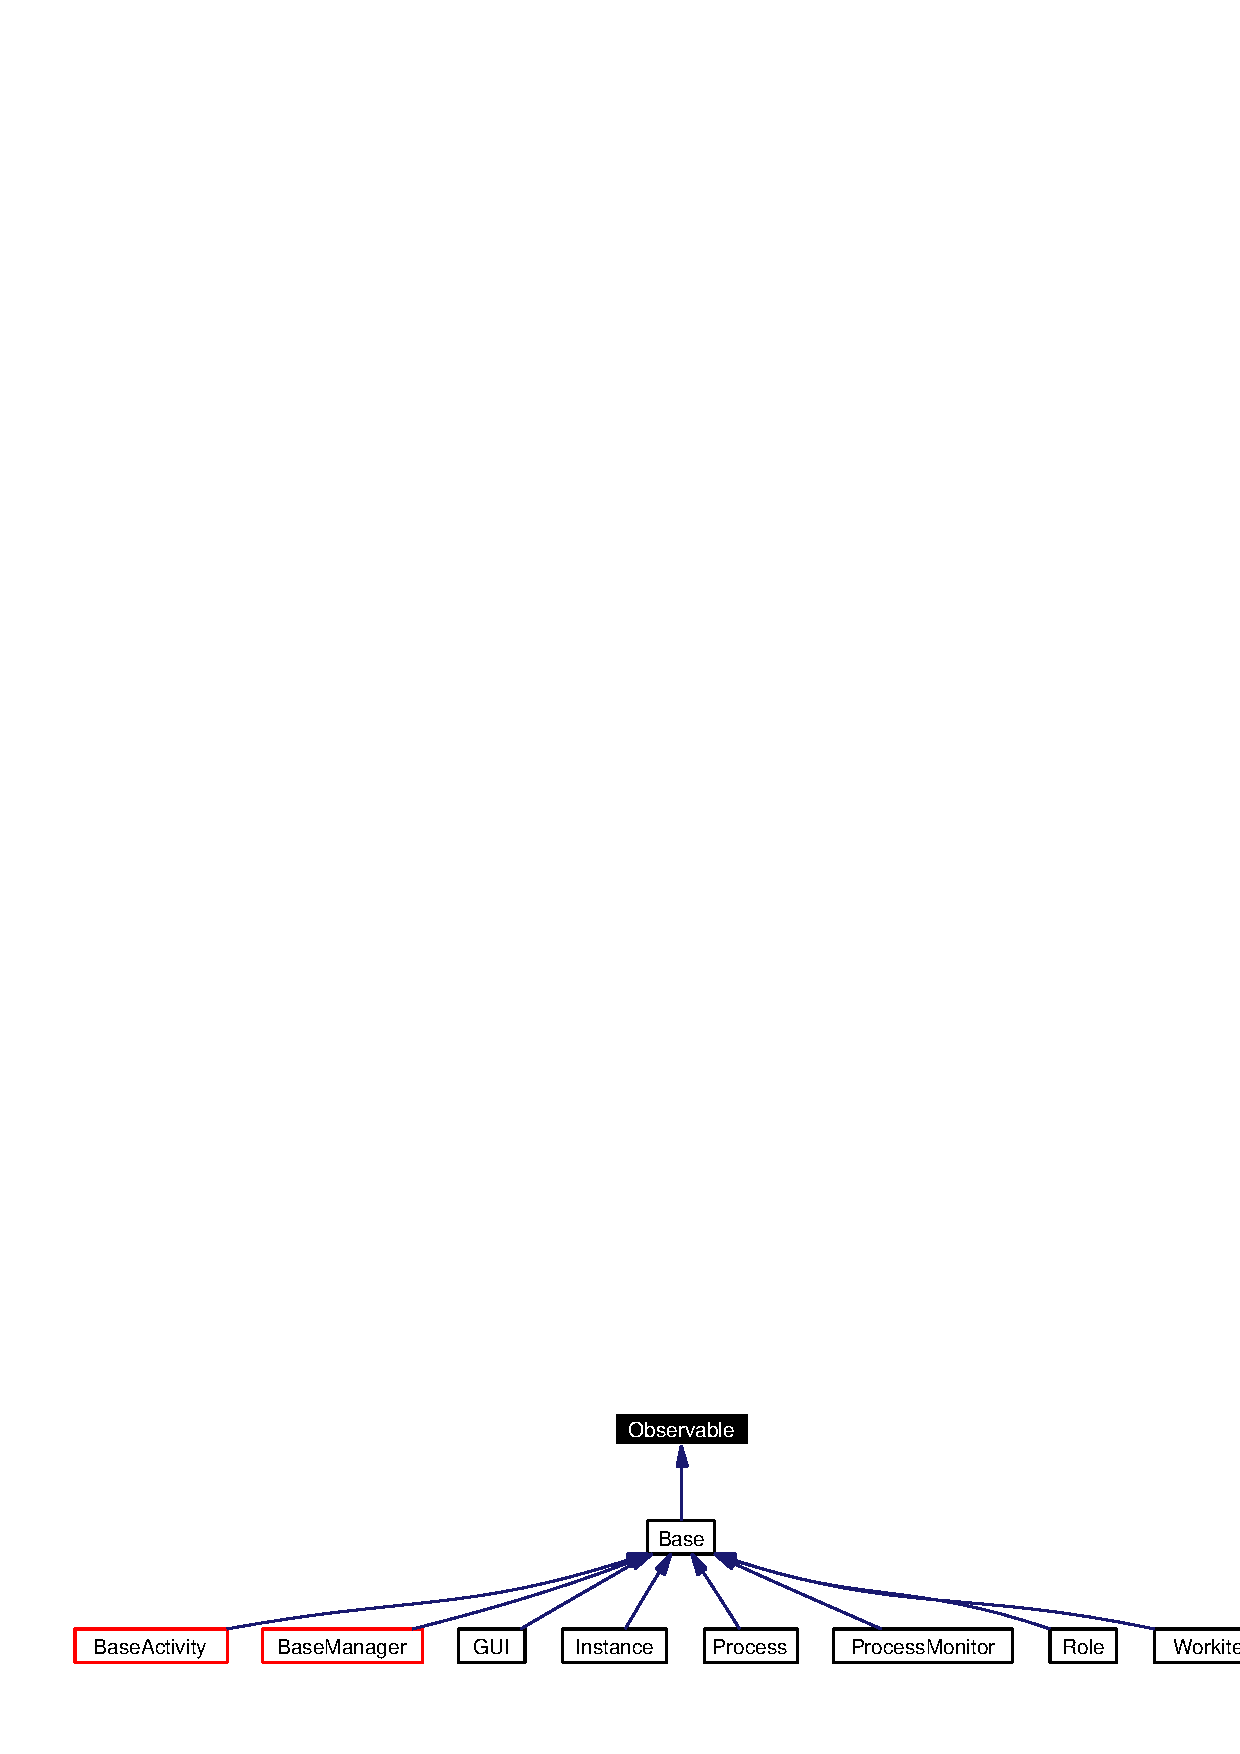
\includegraphics[width=89pt]{classObservable__inherit__graph}
\end{center}
\end{figure}
\subsection*{Public Member Functions}
\begin{CompactItemize}
\item 
{\bf attach} (\$event,\&\$obj)
\item 
{\bf attach\_\-all} (\&\$obj)
\item 
{\bf dettach} (\&\$obj)
\end{CompactItemize}
\subsection*{Public Attributes}
\begin{CompactItemize}
\item 
\index{_observers@{\_\-observers}!Observable@{Observable}}\index{Observable@{Observable}!_observers@{\_\-observers}}
{\bf \_\-observers} = Array()\label{classObservable_m0}

\end{CompactItemize}
\subsection*{Protected Member Functions}
\begin{CompactItemize}
\item 
{\bf notify\_\-all} (\$event,\$msg)
\end{CompactItemize}


\subsection{Detailed Description}
Methods to override: NONE This class implements the {\bf Observer} design pattern defining Observable objects, when a class extends Observable Observers can be attached to the class listening for some event. When an event is detected in any method of the derived class the method can call notify\-All(\$event,\$msg) to notify all the observers listening for event \$event. The {\bf Observer} objects must extend the {\bf Observer} class and define the notify(\$event,\$msg) method. 



Definition at line 15 of file Observable.php.

\subsection{Member Function Documentation}
\index{Observable@{Observable}!attach@{attach}}
\index{attach@{attach}!Observable@{Observable}}
\subsubsection{\setlength{\rightskip}{0pt plus 5cm}Observable::attach (\$ {\em event}, \&\$ {\em obj})}\label{classObservable_a1}


This method can be used to attach an object to the class listening for some specific event. The object will be notified when the specified event is triggered by the derived class. 

Definition at line 27 of file Observable.php.\index{Observable@{Observable}!attach_all@{attach\_\-all}}
\index{attach_all@{attach\_\-all}!Observable@{Observable}}
\subsubsection{\setlength{\rightskip}{0pt plus 5cm}Observable::attach\_\-all (\&\$ {\em obj})}\label{classObservable_a2}


Attaches an object to the class listening for any event. The object will be notified when any event occurs in the derived class. 

Definition at line 40 of file Observable.php.\index{Observable@{Observable}!dettach@{dettach}}
\index{dettach@{dettach}!Observable@{Observable}}
\subsubsection{\setlength{\rightskip}{0pt plus 5cm}Observable::dettach (\&\$ {\em obj})}\label{classObservable_a3}


Detaches an observer from the class. 

Definition at line 52 of file Observable.php.\index{Observable@{Observable}!notify_all@{notify\_\-all}}
\index{notify_all@{notify\_\-all}!Observable@{Observable}}
\subsubsection{\setlength{\rightskip}{0pt plus 5cm}Observable::notify\_\-all (\$ {\em event}, \$ {\em msg})\hspace{0.3cm}{\tt  [protected]}}\label{classObservable_b0}


Method used to notify objects of an event. This is called in the methods of the derived class that want to notify some event. 

Definition at line 64 of file Observable.php.

Referenced by Process\-Manager::activate\_\-process(), Process\-Manager::deactivate\_\-process(), Process\-Manager::import\_\-process(), Process\-Manager::remove\_\-process(), and Process\-Manager::replace\_\-process().

The documentation for this class was generated from the following file:\begin{CompactItemize}
\item 
Observable.php\end{CompactItemize}
